\section{Geometric Image Transformations}

The functions in this section perform various geometrical transformations of 2D images. That is, they do not change the image content, but deform the pixel grid, and map this deformed grid to the destination image. In fact, to avoid sampling artifacts, the mapping is done in the reverse order, from destination to the source. That is, for each pixel $(x, y)$ of the destination image, the functions compute coordinates of the corresponding "donor" pixel in the source image and copy the pixel value, that is:

\[\texttt{dst}(x,y)=\texttt{src}(f_x(x,y), f_y(x,y))\]

In the case when the user specifies the forward mapping: $\left<g_x, g_y\right>: \texttt{src} \rightarrow \texttt{dst}$, the OpenCV functions first compute the corresponding inverse mapping: $\left<f_x, f_y\right>: \texttt{dst} \rightarrow \texttt{src}$ and then use the above formula.

The actual implementations of the geometrical transformations, from the most generic \cvCross{Remap}{remap} and to the simplest and the fastest \cvCross{Resize}{resize}, need to solve the 2 main problems with the above formula:
\begin{enumerate}
    \item extrapolation of non-existing pixels. Similarly to the filtering functions, described in the previous section, for some $(x,y)$ one of $f_x(x,y)$ or $f_y(x,y)$, or they both, may fall outside of the image, in which case some extrapolation method needs to be used. OpenCV provides the same selection of the extrapolation methods as in the filtering functions, but also an additional method \texttt{BORDER\_TRANSPARENT}, which means that the corresponding pixels in the destination image will not be modified at all.
    \item interpolation of pixel values. Usually $f_x(x,y)$ and $f_y(x,y)$ are floating-point numbers (i.e. $\left<f_x, f_y\right>$ can be an affine or perspective transformation, or radial lens distortion correction etc.), so a pixel values at fractional coordinates needs to be retrieved. In the simplest case the coordinates can be just rounded to the nearest integer coordinates and the corresponding pixel used, which is called nearest-neighbor interpolation. However, a better result can be achieved by using more sophisticated \href{http://en.wikipedia.org/wiki/Multivariate_interpolation}{interpolation methods}, where a polynomial function is fit into some neighborhood of the computed pixel $(f_x(x,y), f_y(x,y))$ and then the value of the polynomial at $(f_x(x,y), f_y(x,y))$ is taken as the interpolated pixel value. In OpenCV you can choose between several interpolation methods, see \cvCross{Resize}{resize}. 
\end{enumerate}

\ifCPy

\cvCPyFunc{GetRotationMatrix2D}
Calculates the affine matrix of 2d rotation.

\cvdefC{
CvMat* cv2DRotationMatrix(
\par CvPoint2D32f center,
\par double angle,
\par double scale,
\par CvMat* mapMatrix );
}\cvdefPy{GetRotationMatrix2D(center,angle,scale,mapMatrix)-> None}

\begin{description}
\cvarg{center}{Center of the rotation in the source image}
\cvarg{angle}{The rotation angle in degrees. Positive values mean counter-clockwise rotation (the coordinate origin is assumed to be the top-left corner)}
\cvarg{scale}{Isotropic scale factor}
\cvarg{mapMatrix}{Pointer to the destination $2\times 3$ matrix}
\end{description}

The function \texttt{cv2DRotationMatrix} calculates the following matrix:

\[
\begin{bmatrix}
\alpha & \beta & (1-\alpha) \cdot \texttt{center.x} - \beta \cdot \texttt{center.y} \\
-\beta & \alpha & \beta \cdot \texttt{center.x} - (1-\alpha) \cdot \texttt{center.y}
\end{bmatrix}
\]

where

\[
\alpha = \texttt{scale} \cdot cos(\texttt{angle}), \beta = \texttt{scale} \cdot sin(\texttt{angle})
\]

The transformation maps the rotation center to itself. If this is not the purpose, the shift should be adjusted.

\cvCPyFunc{GetAffineTransform}
Calculates the affine transform from 3 corresponding points.

\cvdefC{
CvMat* cvGetAffineTransform(
\par const CvPoint2D32f* src,
\par const CvPoint2D32f* dst, 
\par CvMat* mapMatrix );
}\cvdefPy{GetAffineTransform(src,dst,mapMatrix)-> None}

\begin{description}
\cvarg{src}{ Coordinates of 3 triangle vertices in the source image}
\cvarg{dst}{ Coordinates of the 3 corresponding triangle vertices in the destination image}
\cvarg{mapMatrix}{ Pointer to the destination $2 \times 3$ matrix}
\end{description}

The function cvGetAffineTransform calculates the matrix of an affine transform such that:

\[
\begin{bmatrix}
x'_i\\
y'_i
\end{bmatrix}
=
\texttt{mapMatrix}
\cdot
\begin{bmatrix}
x_i\\
y_i\\
1
\end{bmatrix}
\]

where

\[
dst(i)=(x'_i,y'_i),
src(i)=(x_i, y_i),
i=0,1,2
\]

\cvCPyFunc{GetPerspectiveTransform}
Calculates the perspective transform from 4 corresponding points.

\cvdefC{
CvMat* cvGetPerspectiveTransform(
\par const CvPoint2D32f* src,
\par const CvPoint2D32f* dst,
\par CvMat* mapMatrix );
}\cvdefPy{GetPerspectiveTransform(src,dst,mapMatrix)-> None}

\begin{description}
\cvarg{src}{Coordinates of 4 quadrangle vertices in the source image}
\cvarg{dst}{Coordinates of the 4 corresponding quadrangle vertices in the destination image}
\cvarg{mapMatrix}{Pointer to the destination $3\times 3$ matrix}
\end{description}

The function \texttt{cvGetPerspectiveTransform} calculates a matrix of perspective transforms such that:

\[
\begin{bmatrix}
x'_i\\
y'_i
\end{bmatrix}
=
\texttt{mapMatrix}
\cdot
\begin{bmatrix}
x_i\\
y_i\\
1
\end{bmatrix}
\]

where

\[
dst(i)=(x'_i,y'_i),
src(i)=(x_i, y_i),
i=0,1,2,3
\]

\cvCPyFunc{GetQuadrangleSubPix}
Retrieves the pixel quadrangle from an image with sub-pixel accuracy.

\cvdefC{
void cvGetQuadrangleSubPix(
\par const CvArr* src,
\par CvArr* dst,
\par const CvMat* mapMatrix );
}\cvdefPy{GetQuadrangleSubPix(src,dst,mapMatrix)-> None}

\begin{description}
\cvarg{src}{Source image}
\cvarg{dst}{Extracted quadrangle}
\cvarg{mapMatrix}{The transformation $2 \times 3$ matrix $[A|b]$ (see the discussion)}
\end{description}

The function \texttt{cvGetQuadrangleSubPix} extracts pixels from \texttt{src} at sub-pixel accuracy and stores them to \texttt{dst} as follows:

\[
dst(x, y)= src( A_{11} x' + A_{12} y' + b_1, A_{21} x' + A_{22} y' + b_2)
\]

where

\[
x'=x-\frac{(width(dst)-1)}{2}, 
y'=y-\frac{(height(dst)-1)}{2}
\]

and

\[
\texttt{mapMatrix} = \begin{bmatrix}
A_{11} & A_{12} & b_1\\
A_{21} & A_{22} & b_2
\end{bmatrix}
\]

The values of pixels at non-integer coordinates are retrieved using bilinear interpolation. When the function needs pixels outside of the image, it uses replication border mode to reconstruct the values. Every channel of multiple-channel images is processed independently.


\cvCPyFunc{GetRectSubPix}
Retrieves the pixel rectangle from an image with sub-pixel accuracy.
 
\cvdefC{void cvGetRectSubPix(
\par const CvArr* src,
\par CvArr* dst,
\par CvPoint2D32f center );
}\cvdefPy{GetRectSubPix(src,dst,center)-> None}

\begin{description}
\cvarg{src}{Source image}
\cvarg{dst}{Extracted rectangle}
\cvarg{center}{Floating point coordinates of the extracted rectangle center within the source image. The center must be inside the image}
\end{description}

The function \texttt{cvGetRectSubPix} extracts pixels from \texttt{src}:

\[
dst(x, y) = src(x + \texttt{center.x} - (width(\texttt{dst})-1)*0.5, y + \texttt{center.y} - (height(\texttt{dst} )-1)*0.5)
\]

where the values of the pixels at non-integer coordinates are retrieved
using bilinear interpolation. Every channel of multiple-channel
images is processed independently. While the rectangle center
must be inside the image, parts of the rectangle may be
outside. In this case, the replication border mode is used to get
pixel values beyond the image boundaries.


\cvCPyFunc{LogPolar}
Remaps an image to log-polar space.

\cvdefC{
void cvLogPolar(
\par const CvArr* src,
\par CvArr* dst,
\par CvPoint2D32f center,
\par double M,
\par int flags=CV\_INTER\_LINEAR+CV\_WARP\_FILL\_OUTLIERS );}
\cvdefPy{LogPolar(src,dst,center,M,flags=CV\_INNER\_LINEAR+CV\_WARP\_FILL\_OUTLIERS)-> None}

\begin{description}
\cvarg{src}{Source image}
\cvarg{dst}{Destination image}
\cvarg{center}{The transformation center; where the output precision is maximal}
\cvarg{M}{Magnitude scale parameter. See below}
\cvarg{flags}{A combination of interpolation methods and the following optional flags:
\begin{description}
  \cvarg{CV\_WARP\_FILL\_OUTLIERS}{fills all of the destination image pixels. If some of them correspond to outliers in the source image, they are set to zero}
  \cvarg{CV\_WARP\_INVERSE\_MAP}{See below}
\end{description}}
\end{description}

The function \texttt{cvLogPolar} transforms the source image using the following transformation:

Forward transformation (\texttt{CV\_WARP\_INVERSE\_MAP} is not set):

\[
dst(\phi,\rho) = src(x,y)
\]

Inverse transformation (\texttt{CV\_WARP\_INVERSE\_MAP} is set):

\[
dst(x,y) = src(\phi,\rho)
\]

where

\[
\rho = M \cdot \log{\sqrt{x^2 + y^2}},
\phi=atan(y/x)
\]

The function emulates the human "foveal" vision and can be used for fast scale and rotation-invariant template matching, for object tracking and so forth.
The function can not operate in-place.

\ifC
% Example: Log-polar transformation
\begin{lstlisting}
#include <cv.h>
#include <highgui.h>

int main(int argc, char** argv)
{
    IplImage* src;

    if( argc == 2 && (src=cvLoadImage(argv[1],1) != 0 )
    {
        IplImage* dst = cvCreateImage( cvSize(256,256), 8, 3 );
        IplImage* src2 = cvCreateImage( cvGetSize(src), 8, 3 );
        cvLogPolar( src, dst, cvPoint2D32f(src->width/2,src->height/2), 40, 
        CV_INTER_LINEAR+CV_WARP_FILL_OUTLIERS );
        cvLogPolar( dst, src2, cvPoint2D32f(src->width/2,src->height/2), 40, 
        CV_INTER_LINEAR+CV_WARP_FILL_OUTLIERS+CV_WARP_INVERSE_MAP );
        cvNamedWindow( "log-polar", 1 );
        cvShowImage( "log-polar", dst );
        cvNamedWindow( "inverse log-polar", 1 );
        cvShowImage( "inverse log-polar", src2 );
        cvWaitKey();
    }
    return 0;
}
\end{lstlisting}

And this is what the program displays when \texttt{opencv/samples/c/fruits.jpg} is passed to it
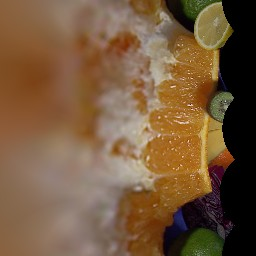
\includegraphics[width=0.4\textwidth]{pics/logpolar.jpg}
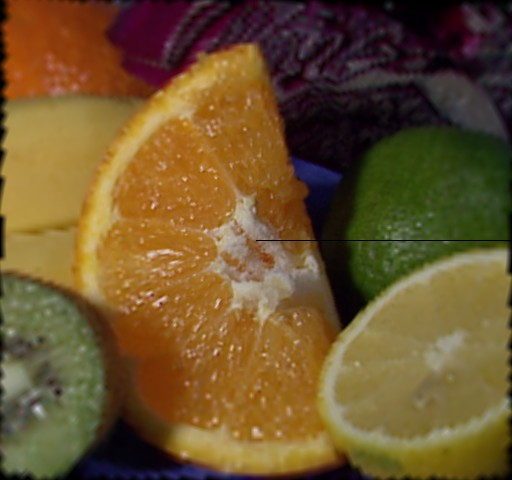
\includegraphics[width=0.4\textwidth]{pics/inv_logpolar.jpg}
\fi

\cvCPyFunc{Remap}
Applies a generic geometrical transformation to the image.

\cvdefC{
void cvRemap(
\par const CvArr* src,
\par CvArr* dst,
\par const CvArr* mapx,
\par const CvArr* mapy,
\par int flags=CV\_INTER\_LINEAR+CV\_WARP\_FILL\_OUTLIERS,
\par CvScalar fillval=cvScalarAll(0) );}
\cvdefPy{Remap(src,dst,mapx,mapy,flags=CV\_INNER\_LINEAR+CV\_WARP\_FILL\_OUTLIERS,fillval=(0,0,0,0))-> None}

\begin{description}
\cvarg{src}{Source image}
\cvarg{dst}{Destination image}
\cvarg{mapx}{The map of x-coordinates (CV\_32FC1 image)}
\cvarg{mapy}{The map of y-coordinates (CV\_32FC1 image)}
\cvarg{flags}{A combination of interpolation method and the following optional flag(s):
\begin{description}
  \cvarg{CV\_WARP\_FILL\_OUTLIERS}{fills all of the destination image pixels. If some of them correspond to outliers in the source image, they are set to \texttt{fillval}}
\end{description}}
\cvarg{fillval}{A value used to fill outliers}
\end{description}

The function \texttt{cvRemap} transforms the source image using the specified map:

\[
\texttt{dst}(x,y) = \texttt{src}(\texttt{mapx}(x,y),\texttt{mapy}(x,y))
\]

Similar to other geometrical transformations, some interpolation method (specified by user) is used to extract pixels with non-integer coordinates.
Note that the function can not operate in-place.

\cvCPyFunc{Resize}
Resizes an image.

\cvdefC{
void cvResize(
\par const CvArr* src,
\par CvArr* dst,
\par int interpolation=CV\_INTER\_LINEAR );}
\cvdefPy{Resize(src,dst,interpolation=CV\_INTER\_LINEAR)-> None}

\begin{description}
\cvarg{src}{Source image}
\cvarg{dst}{Destination image}
\cvarg{interpolation}{Interpolation method:
\begin{description}
\cvarg{CV\_INTER\_NN}{nearest-neigbor interpolation}
\cvarg{CV\_INTER\_LINEAR}{bilinear interpolation (used by default)}
\cvarg{CV\_INTER\_AREA}{resampling using pixel area relation. It is the preferred method for image decimation that gives moire-free results. In terms of zooming it is similar to the \texttt{CV\_INTER\_NN} method}
\cvarg{CV\_INTER\_CUBIC}{bicubic interpolation}
\end{description}}
\end{description}

The function \texttt{cvResize} resizes an image \texttt{src} so that it fits exactly into \texttt{dst}. If ROI is set, the function considers the ROI as supported.


\cvCPyFunc{WarpAffine}
Applies an affine transformation to an image.

\cvdefC{
void cvWarpAffine(
\par const CvArr* src,
\par CvArr* dst,
\par const CvMat* mapMatrix,
\par int flags=CV\_INTER\_LINEAR+CV\_WARP\_FILL\_OUTLIERS,
\par CvScalar fillval=cvScalarAll(0) );
}
\cvdefPy{WarpAffine(src,dst,mapMatrix,flags=CV\_INTER\_LINEAR+CV\_WARP\_FILL\_OUTLIERS,fillval=(0,0,0,0))-> None}

\begin{description}
\cvarg{src}{Source image}
\cvarg{dst}{Destination image}
\cvarg{mapMatrix}{$2\times 3$ transformation matrix}
\cvarg{flags}{A combination of interpolation methods and the following optional flags:
\begin{description}
  \cvarg{CV\_WARP\_FILL\_OUTLIERS}{fills all of the destination image pixels; if some of them correspond to outliers in the source image, they are set to \texttt{fillval}}
  \cvarg{CV\_WARP\_INVERSE\_MAP}{indicates that \texttt{matrix} is inversely
  transformed from the destination image to the source and, thus, can be used
  directly for pixel interpolation. Otherwise, the function finds
  the inverse transform from \texttt{mapMatrix}}}
\end{description}
\cvarg{fillval}{A value used to fill outliers}
\end{description}

The function \texttt{cvWarpAffine} transforms the source image using the specified matrix:

\[
dst(x',y') = src(x,y)
\]

where

\[
\begin{matrix}
\begin{bmatrix}
x'\\
y'
\end{bmatrix} = \texttt{mapMatrix} \cdot \begin{bmatrix}
x\\
y\\
1
\end{bmatrix} & \mbox{if CV\_WARP\_INVERSE\_MAP is not set}\\
\begin{bmatrix}
x\\
y
\end{bmatrix} = \texttt{mapMatrix} \cdot \begin{bmatrix}
x'\\
y'\\
1
\end{bmatrix}& \mbox{otherwise}
\end{matrix}
\]

The function is similar to \cvCPyCross{GetQuadrangleSubPix} but they are not exactly the same. \cvCPyCross{WarpAffine} requires input and output image have the same data type, has larger overhead (so it is not quite suitable for small images) and can leave part of destination image unchanged. While \cvCPyCross{GetQuadrangleSubPix} may extract quadrangles from 8-bit images into floating-point buffer, has smaller overhead and always changes the whole destination image content.
Note that the function can not operate in-place.

To transform a sparse set of points, use the \cvCPyCross{Transform} function from cxcore.

\cvCPyFunc{WarpPerspective}
Applies a perspective transformation to an image.

\cvdefC{
void cvWarpPerspective(
\par const CvArr* src,
\par CvArr* dst,
\par const CvMat* mapMatrix,
\par int flags=CV\_INTER\_LINEAR+CV\_WARP\_FILL\_OUTLIERS,
\par CvScalar fillval=cvScalarAll(0) );
}
\cvdefPy{WarpPerspective(src,dst,mapMatrix,flags=CV\_INNER\_LINEAR+CV\_WARP\_FILL\_OUTLIERS,fillval=(0,0,0,0))-> None}

\begin{description}
\cvarg{src}{Source image}
\cvarg{dst}{Destination image}
\cvarg{mapMatrix}{$3\times 3$ transformation matrix}
\cvarg{flags}{A combination of interpolation methods and the following optional flags:
\begin{description}
  \cvarg{CV\_WARP\_FILL\_OUTLIERS}{fills all of the destination image pixels; if some of them correspond to outliers in the source image, they are set to \texttt{fillval}}
  \cvarg{CV\_WARP\_INVERSE\_MAP}{indicates that \texttt{matrix} is inversely transformed from the destination image to the source and, thus, can be used directly for pixel interpolation. Otherwise, the function finds the inverse transform from \texttt{mapMatrix}}
\end{description}}
\cvarg{fillval}{A value used to fill outliers}
\end{description}

The function \texttt{cvWarpPerspective} transforms the source image using the specified matrix:

\[
\begin{matrix}
\begin{bmatrix}
x'\\
y'
\end{bmatrix} = \texttt{mapMatrix} \cdot \begin{bmatrix}
x\\
y\\
1
\end{bmatrix} & \mbox{if CV\_WARP\_INVERSE\_MAP is not set}\\
\begin{bmatrix}
x\\
y
\end{bmatrix} = \texttt{mapMatrix} \cdot \begin{bmatrix}
x'\\
y'\\
1
\end{bmatrix}& \mbox{otherwise}
\end{matrix}
\]

Note that the function can not operate in-place.
For a sparse set of points use the \cvCPyCross{PerspectiveTransform} function from CxCore.

\fi

\ifCpp

\cvCppFunc{convertMaps}
Converts image transformation maps from one representation to another

\cvdefCpp{void convertMaps( const Mat\& map1, const Mat\& map2,\par
                  Mat\& dstmap1, Mat\& dstmap2,\par
                  int dstmap1type, bool nninterpolation=false );}
\begin{description}
\cvarg{map1}{The first input map of type \texttt{CV\_16SC2} or \texttt{CV\_32FC1} or \texttt{CV\_32FC2}}
\cvarg{map2}{The second input map of type \texttt{CV\_16UC1} or \texttt{CV\_32FC1} or none (empty matrix), respectively}
\cvarg{dstmap1}{The first output map; will have type \texttt{dstmap1type} and the same size as \texttt{src}}
\cvarg{dstmap2}{The second output map}
\cvarg{dstmap1type}{The type of the first output map; should be \texttt{CV\_16SC2}, \texttt{CV\_32FC1} or \texttt{CV\_32FC2}}
\cvarg{nninterpolation}{Indicates whether the fixed-point maps will be used for nearest-neighbor or for more complex interpolation}
\end{description}

The function converts a pair of maps for \cvCppCross{remap} from one representation to another. The following options (\texttt{(map1.type(), map2.type())} $\rightarrow$ \texttt{(dstmap1.type(), dstmap2.type())}) are supported:
\begin{enumerate}
    \item $\texttt{(CV\_32FC1, CV\_32FC1)} \rightarrow \texttt{(CV\_16SC2, CV\_16UC1)}$. This is the most frequently used conversion operation, in which the original floating-point maps (see \cvCppCross{remap}) are converted to more compact and much faster fixed-point representation. The first output array will contain the rounded coordinates and the second array (created only when \texttt{nninterpolation=false}) will contain indices in the interpolation tables.   
    \item $\texttt{(CV\_32FC2)} \rightarrow \texttt{(CV\_16SC2, CV\_16UC1)}$. The same as above, but the original maps are stored in one 2-channel matrix.
    \item the reverse conversion. Obviously, the reconstructed floating-point maps will not be exactly the same as the originals.
\end{enumerate} 

See also: \cvCppCross{remap}, \cvCppCross{undisort}, \cvCppCross{initUndistortRectifyMap}

\cvCppFunc{getAffineTransform}
Calculates the affine transform from 3 pairs of the corresponding points

\cvdefCpp{Mat getAffineTransform( const Point2f src[], const Point2f dst[] );}

\begin{description}
\cvarg{src}{Coordinates of a triangle vertices in the source image}
\cvarg{dst}{Coordinates of the corresponding triangle vertices in the destination image}
\end{description}

The function calculates the $2 \times 3$ matrix of an affine transform such that:

\[
\begin{bmatrix}
x'_i\\
y'_i
\end{bmatrix}
=
\texttt{map\_matrix}
\cdot
\begin{bmatrix}
x_i\\
y_i\\
1
\end{bmatrix}
\]

where

\[
dst(i)=(x'_i,y'_i),
src(i)=(x_i, y_i),
i=0,1,2
\]

See also: \cvCppCross{warpAffine}, \cvCppCross{transform}

\cvCppFunc{getPerspectiveTransform}
Calculates the perspective transform from 4 pairs of the corresponding points

\cvdefCpp{Mat getPerspectiveTransform( const Point2f src[], \par const Point2f dst[] );}

\begin{description}
\cvarg{src}{Coordinates of a quadrange vertices in the source image}
\cvarg{dst}{Coordinates of the corresponding quadrangle vertices in the destination image}
\end{description}

The function calculates the $3 \times 3$ matrix of a perspective transform such that:

\[
\begin{bmatrix}
t_i x'_i\\
t_i y'_i\\
t_i
\end{bmatrix}
=
\texttt{map\_matrix}
\cdot
\begin{bmatrix}
x_i\\
y_i\\
1
\end{bmatrix}
\]

where

\[
dst(i)=(x'_i,y'_i),
src(i)=(x_i, y_i),
i=0,1,2
\]

See also: \cvCppCross{findHomography}, \cvCppCross{warpPerspective}, \cvCppCross{perspectiveTransform}

\cvCppFunc{getRectSubPix}
Retrieves the pixel rectangle from an image with sub-pixel accuracy

\cvdefCpp{void getRectSubPix( const Mat\& image, Size patchSize,\par
                    Point2f center, Mat\& dst, int patchType=-1 );}
\begin{description}
\cvarg{src}{Source image}
\cvarg{patchSize}{Size of the extracted patch}
\cvarg{center}{Floating point coordinates of the extracted rectangle center within the source image. The center must be inside the image}
\cvarg{dst}{The extracted patch; will have the size \texttt{patchSize} and the same number of channels as \texttt{src}}
\cvarg{patchType}{The depth of the extracted pixels. By default they will have the same depth as \texttt{src}}
\end{description}

The function \texttt{getRectSubPix} extracts pixels from \texttt{src}:

\[
dst(x, y) = src(x + \texttt{center.x} - (\texttt{dst.cols}-1)*0.5, y + \texttt{center.y} - (\texttt{dst.rows}-1)*0.5)
\]

where the values of the pixels at non-integer coordinates are retrieved
using bilinear interpolation. Every channel of multiple-channel
images is processed independently. While the rectangle center
must be inside the image, parts of the rectangle may be
outside. In this case, the replication border mode (see \cvCppCross{borderInterpolate}) is used to extrapolate
the pixel values outside of the image.

See also: \cvCppCross{warpAffine}, \cvCppCross{warpPerspective}

\cvCppFunc{getRotationMatrix2D}
Calculates the affine matrix of 2d rotation.

\cvdefCpp{Mat getRotationMatrix2D( Point2f center, double angle, double scale );}
\begin{description}
\cvarg{center}{Center of the rotation in the source image}
\cvarg{angle}{The rotation angle in degrees. Positive values mean counter-clockwise rotation (the coordinate origin is assumed to be the top-left corner)}
\cvarg{scale}{Isotropic scale factor}
\end{description}

The function calculates the following matrix:

\[
\begin{bmatrix}
\alpha & \beta & (1-\alpha) \cdot \texttt{center.x} - \beta \cdot \texttt{center.y} \\
-\beta & \alpha & \beta \cdot \texttt{center.x} - (1-\alpha) \cdot \texttt{center.y}
\end{bmatrix}
\]

where

\[
\begin{array}{l}
\alpha = \texttt{scale} \cdot \cos \texttt{angle},\\
\beta = \texttt{scale} \cdot \sin \texttt{angle}
\end{array}
\]

The transformation maps the rotation center to itself. If this is not the purpose, the shift should be adjusted.

See also: \cvCppCross{getAffineTransform}, \cvCppCross{warpAffine}, \cvCppCross{transform}


\cvCppFunc{invertAffineTransform}
Inverts an affine transformation

\cvdefCpp{void invertAffineTransform(const Mat\& M, Mat\& iM);}
\begin{description}
\cvarg{M}{The original affine transformation}
\cvarg{iM}{The output reverse affine transformation}
\end{description}

The function computes inverse affine transformation represented by $2 \times 3$ matrix \texttt{M}:

\[\begin{bmatrix}
a_{11} & a_{12} & b_1 \\
a_{21} & a_{22} & b_2
\end{bmatrix}
\]

The result will also be a $2 \times 3$ matrix of the same type as \texttt{M}.

\cvCppFunc{remap}
Applies a generic geometrical transformation to an image.

\cvdefCpp{void remap( const Mat\& src, Mat\& dst, const Mat\& map1, const Mat\& map2,\par
            int interpolation, int borderMode=BORDER\_CONSTANT,\par
            const Scalar\& borderValue=Scalar());}
\begin{description}
\cvarg{src}{Source image}
\cvarg{dst}{Destination image. It will have the same size as \texttt{map1} and the same type as \texttt{src}}
\cvarg{map1}{The first map of either \texttt{(x,y)} points or just \texttt{x} values having type \texttt{CV\_16SC2}, \texttt{CV\_32FC1} or \texttt{CV\_32FC2}. See \cvCppCross{convertMaps} for converting floating point representation to fixed-point for speed.}
\cvarg{map2}{The second map of \texttt{y} values having type \texttt{CV\_16UC1}, \texttt{CV\_32FC1} or none (empty map if map1 is \texttt{(x,y)} points), respectively}
\cvarg{interpolation}{The interpolation method, see \cvCppCross{resize}. The method \texttt{INTER\_AREA} is not supported by this function}
\cvarg{borderMode}{The pixel extrapolation method, see \cvCppCross{borderInterpolate}. When the\\ \texttt{borderMode=BORDER\_TRANSPARENT}, it means that the pixels in the destination image that corresponds to the "outliers" in the source image are not modified by the function}
\cvarg{borderValue}{A value used in the case of a constant border. By default it is 0}
\end{description}

The function \texttt{remap} transforms the source image using the specified map:

\[
\texttt{dst}(x,y) = \texttt{src}(map_x(x,y),map_y(x,y))
\]

Where values of pixels with non-integer coordinates are computed using one of the available interpolation methods. $map_x$ and $map_y$ 
can be encoded as separate floating-point maps in $map_1$ and $map_2$ respectively, or interleaved floating-point maps of $(x,y)$ in $map_1$, or 
fixed-point maps made by using \cvCppCross{convertMaps}. The reason you might want to convert from floating to fixed-point 
representations of a map is that they can yield much faster (~2x) remapping operations. In the converted case, $map_1$ contains pairs 
\texttt{(cvFloor(x), cvFloor(y))} and $map_2$ contains indices in a table of interpolation coefficients. 

This function can not operate in-place.

\cvCppFunc{resize}
Resizes an image

\cvdefCpp{void resize( const Mat\& src, Mat\& dst,\par
             Size dsize, double fx=0, double fy=0,\par
             int interpolation=INTER\_LINEAR );}
\begin{description}
\cvarg{src}{Source image}
\cvarg{dst}{Destination image. It will have size \texttt{dsize} (when it is non-zero) or the size computed from \texttt{src.size()}
and \texttt{fx} and \texttt{fy}. The type of \texttt{dst} will be the same as of \texttt{src}.}
\cvarg{dsize}{The destination image size. If it is zero, then it is computed as:
\[\texttt{dsize = Size(round(fx*src.cols), round(fy*src.rows))}\].
Either \texttt{dsize} or both \texttt{fx} or \texttt{fy} must be non-zero.}
\cvarg{fx}{The scale factor along the horizontal axis. When 0, it is computed as
\[\texttt{(double)dsize.width/src.cols}\]}
\cvarg{fy}{The scale factor along the vertical axis. When 0, it is computed as
\[\texttt{(double)dsize.height/src.rows}\]}
\cvarg{interpolation}{The interpolation method:
\begin{description}
\cvarg{INTER\_NEAREST}{nearest-neighbor interpolation}
\cvarg{INTER\_LINEAR}{bilinear interpolation (used by default)}
\cvarg{INTER\_AREA}{resampling using pixel area relation. It may be the preferred method for image decimation, as it gives moire-free results. But when the image is zoomed, it is similar to the \texttt{INTER\_NEAREST} method}
\cvarg{INTER\_CUBIC}{bicubic interpolation over 4x4 pixel neighborhood}
\cvarg{INTER\_LANCZOS4}{Lanczos interpolation over 8x8 pixel neighborhood}
\end{description}}
\end{description}

The function \texttt{resize} resizes an image \texttt{src} down to or up to the specified size.
Note that the initial \texttt{dst} type or size are not taken into account. Instead the size and type are derived from the \texttt{src}, \texttt{dsize}, \texttt{fx} and \texttt{fy}. If you want to resize \texttt{src} so that it fits the pre-created \texttt{dst}, you may call the function as:

\begin{lstlisting}
// explicitly specify dsize=dst.size(); fx and fy will be computed from that.
resize(src, dst, dst.size(), 0, 0, interpolation);
\end{lstlisting}

If you want to decimate the image by factor of 2 in each direction, you can call the function this way:

\begin{lstlisting}
// specify fx and fy and let the function to compute the destination image size.
resize(src, dst, Size(), 0.5, 0.5, interpolation);
\end{lstlisting}

See also: \cvCppCross{warpAffine}, \cvCppCross{warpPerspective}, \cvCppCross{remap}.


\cvCppFunc{warpAffine}
Applies an affine transformation to an image.

\cvdefCpp{void warpAffine( const Mat\& src, Mat\& dst,\par
                 const Mat\& M, Size dsize,\par
                 int flags=INTER\_LINEAR,\par
                 int borderMode=BORDER\_CONSTANT,\par
                 const Scalar\& borderValue=Scalar());}
\begin{description}
\cvarg{src}{Source image}
\cvarg{dst}{Destination image; will have size \texttt{dsize} and the same type as \texttt{src}}
\cvarg{M}{$2\times 3$ transformation matrix}
\cvarg{dsize}{Size of the destination image}
\cvarg{flags}{A combination of interpolation methods, see \cvCppCross{resize}, and the optional flag \texttt{WARP\_INVERSE\_MAP} that means that \texttt{M} is the inverse transformation ($\texttt{dst}\rightarrow\texttt{src}$)}
\cvarg{borderMode}{The pixel extrapolation method, see \cvCppCross{borderInterpolate}. When the \\ \texttt{borderMode=BORDER\_TRANSPARENT}, it means that the pixels in the destination image that corresponds to the "outliers" in the source image are not modified by the function}
\cvarg{borderValue}{A value used in case of a constant border. By default it is 0}
\end{description}

The function \texttt{warpAffine} transforms the source image using the specified matrix:

\[
\texttt{dst}(x,y) = \texttt{src}(\texttt{M}_{11} x + \texttt{M}_{12} y + \texttt{M}_{13}, \texttt{M}_{21} x + \texttt{M}_{22} y + \texttt{M}_{23})
\]
when the flag \texttt{WARP\_INVERSE\_MAP} is set. Otherwise, the transformation is first inverted with \cvCppCross{invertAffineTransform} and then put in the formula above instead of \texttt{M}.
The function can not operate in-place.

See also: \cvCppCross{warpPerspective}, \cvCppCross{resize}, \cvCppCross{remap}, \cvCppCross{getRectSubPix}, \cvCppCross{transform}

\cvCppFunc{warpPerspective}
Applies a perspective transformation to an image.

\cvdefCpp{void warpPerspective( const Mat\& src, Mat\& dst,\par
                      const Mat\& M, Size dsize,\par
                      int flags=INTER\_LINEAR,\par
                      int borderMode=BORDER\_CONSTANT,\par
                      const Scalar\& borderValue=Scalar());}
\begin{description}
\cvarg{src}{Source image}
\cvarg{dst}{Destination image; will have size \texttt{dsize} and the same type as \texttt{src}}
\cvarg{M}{$3\times 3$ transformation matrix}
\cvarg{dsize}{Size of the destination image}
\cvarg{flags}{A combination of interpolation methods, see \cvCppCross{resize}, and the optional flag \texttt{WARP\_INVERSE\_MAP} that means that \texttt{M} is the inverse transformation ($\texttt{dst}\rightarrow\texttt{src}$)}
\cvarg{borderMode}{The pixel extrapolation method, see \cvCppCross{borderInterpolate}. When the \\ \texttt{borderMode=BORDER\_TRANSPARENT}, it means that the pixels in the destination image that corresponds to the "outliers" in the source image are not modified by the function}
\cvarg{borderValue}{A value used in case of a constant border. By default it is 0}
\end{description}

The function \texttt{warpPerspective} transforms the source image using the specified matrix:

\[
\texttt{dst}(x,y) = \texttt{src}\left(\frac{M_{11} x + M_{12} y + M_{13}}{M_{31} x + M_{32} y + M_{33}},
    \frac{M_{21} x + M_{22} y + M_{23}}{M_{31} x + M_{32} y + M_{33}}\right)
\]
when the flag \texttt{WARP\_INVERSE\_MAP} is set. Otherwise, the transformation is first inverted with \cvCppCross{invert} and then put in the formula above instead of \texttt{M}.
The function can not operate in-place.

See also: \cvCppCross{warpAffine}, \cvCppCross{resize}, \cvCppCross{remap}, \cvCppCross{getRectSubPix}, \cvCppCross{perspectiveTransform}

\fi

